\documentclass[t]{beamer}

\usepackage{etex}
%\documentclass[notes,t]{beamer}

\setbeamertemplate{bibliography item}[text] %default is an icon of an

%\usepackage{mathchars}
\usepackage{amsmath}
\usepackage{mathtools}

\usepackage{booktabs}
\usepackage{float}              %for forcefully placing diagrams 
\usepackage{subcaption}

\usepackage{algorithm}
\usepackage{algpseudocode}
\newcommand{\tab}[1]{\hspace{.08\textwidth}{#1}} % indent tab for data
                                                  % structs in algos
 \newcommand{\LineIf}[3]{ {#1}
   \algorithmicif\ {#2}
   \algorithmicelse\ {#3} } % inline X if Y else Z

\definecolor{oblack}{HTML}{0D1B2E}
\definecolor{deepblue}{HTML}{183152}
\definecolor{navyblue}{HTML}{375D81}
\definecolor{bluegreen}{HTML}{ABC8E2}
\definecolor{beige}{HTML}{C4D7ED}
\definecolor{cream}{HTML}{E1E6FA}
\definecolor{owhite}{HTML}{F9FFFF}
\definecolor{redi}{HTML}{A5121E}
\definecolor{greeni}{HTML}{3E700F}
\newcommand{\hilight}[1]{\colorbox{bluegreen}{#1}}

\setbeamercolor{normal text}{fg=oblack}
\setbeamercolor{alerted text}{fg=redi}
\setbeamercolor{background canvas}{bg=owhite}
%\setbeamercolor{block body alerted}{bg=normal text.bg!90!black}
%\setbeamercolor{block body}{bg=normal text.bg!90!black}
%\setbeamercolor{block body example}{bg=normal text.bg!90!black}
%\setbeamercolor{block title alerted}{use={normal text,alerted text},fg=alerted text.fg!75!normal text.fg,bg=normal text.bg!75!black}
\setbeamercolor{block title}{fg=deepblue}
%\setbeamercolor{block title example}{use={normal text,example text},fg=example text.fg!75!normal text.fg,bg=normal text.bg!75!black}
%\setbeamercolor{fine separation line}{}
\setbeamercolor{frametitle}{fg=navyblue}
%\setbeamercolor{item projected}{fg=black}
%\setbeamercolor{normal text}{bg=black,fg=yellow}
%\setbeamercolor{palette sidebar primary}{use=normal text,fg=normal text.fg}
%\setbeamercolor{palette sidebar quaternary}{use=structure,fg=structure.fg}
%\setbeamercolor{palette sidebar secondary}{use=structure,fg=structure.fg}
%\setbeamercolor{palette sidebar tertiary}{use=normal text,fg=normal text.fg}
\setbeamercolor{section in sidebar}{fg=beige}
\setbeamercolor{section in sidebar shaded}{fg=cream}
%\setbeamercolor{separation line}{}
\setbeamercolor{sidebar}{bg=deepblue}
\setbeamercolor{sidebar left}{bg=deepblue}
\setbeamercolor{author in sidebar}{fg=owhite}
\setbeamercolor{title in sidebar}{fg=owhite}
%\setbeamercolor{sidebar}{parent=palette primary}
%\setbeamercolor{structure}{bg=black, fg=green}
\setbeamercolor{subsection in sidebar}{fg=owhite}
\setbeamercolor{subsection in sidebar shaded}{fg=owhite}
\setbeamercolor{title}{fg=deepblue}
\setbeamercolor{titlelike}{fg=deepblue}
\setbeamercolor{section in toc}{fg=navyblue}
\setbeamercolor{subsection in toc}{fg=bluegreen}
\setbeamercolor{section number projected}{bg=navyblue,fg=cream}
\setbeamercolor{itemize item}{fg=navyblue}
\setbeamercolor{block title alerted}{fg=redi}
\setbeamercolor{block title example}{fg=greeni}
\setbeamercolor{figure caption name}{fg=redi}
\setbeamercolor{figure caption}{fg=redi}
\setbeamercolor{description item}{bg=deepblue,fg=deepblue}

\captionsetup[figure]{labelfont={color=redi,footnotesize},textfont={footnotesize,color=oblack}}

\usepackage{pgfplots}
\usepackage{tikz}
\usetikzlibrary{shapes,
  arrows,
  chains,
  matrix,
  positioning,
  fit,
  scopes,
  calc,
  decorations.pathmorphing}
\makeatletter
\tikzset{join/.code=\tikzset{after node path={%
\ifx\tikzchainprevious\pgfutil@empty\else(\tikzchainprevious)%
edge[every join]#1(\tikzchaincurrent)\fi}}}
\makeatother
\tikzset{>=stealth',every on chain/.append style={join},
         every join/.style={->},
         snake it/.style={decorate, decoration=snake}}
\tikzstyle{labeled}=[execute at begin node=$\scriptstyle,
   execute at end node=$]

\AtBeginSection[]
{
  \begin{frame}
    \tableofcontents[currentsection]
  \end{frame}
}

\usepackage[utf8]{inputenc}
\usetheme{Hannover}
\usecolortheme{dolphin}

\begin{document}

\title[Analysis of Wikipedia hitories] % (optional, only for long titles)
{Automatically defining collaborative share through
    the automatic, na\"ive string analysis of Wikipedia article
    revision histories}
\author % (optional, for multiple authors)
{W~Marsey}
\institute{Imperial College London} % (optional)
\date % (optional)
{Sep 2014}
\subject{Computing Science}

\frame{\titlepage}

\section{Introduction}
  %%%%%%%%%%%%%%%%%%%%%%%%%%%%%%%%%%%%%%%%%%%%%%%%%%
  %%%%%%%%%%%%%%%%%%%%%%%%%%%%%%%%%%%%%%%%%%%%%%%%%%
  %%%%% 
  %%%%% INTRODUCTION
  %%%%%
  %%%%%%%%%%%%%%%%%%%%%%%%%%%%%%%%%%%%%%%%%%%%%%%%%%
  %%%%%%%%%%%%%%%%%%%%%%%%%%%%%%%%%%%%%%%%%%%%%%%%%%


  
  %%%%%%%%%%%%%%%%%%%%%%%%%%%%%%%%%%%%%%%%%%%%%%%%%%
  %%%%% COPYRIGHT
  %%%%%%%%%%%%%%%%%%%%%%%%%%%%%%%%%%%%%%%%%%%%%%%%%%
  \subsection{Copyright legislation}
  \begin{frame}[shrink]
    \setbeamercovered{transparent}

    \frametitle{On copyright} 
    \framesubtitle{What does existing legislature say?}
    \only<1>{
      
      \begin{quote} When two or more authors prepare a work
        with the intent to combine their contributions into
        inseparable or interdependent parts, the work is considered
        joint work and the authors are considered joint copyright
        owners. (UK Intellectual Property
        Office) \cite{what-joint-authorship}
      \end{quote}

    }
    
    \only<1>{

      \begin{quote} Where two or more people have created a
        single work protected by copyright and the contribution of
        each author is not distinct from that of the
        other(s).(Stanford: Copyright \& Fair
        Use) \cite{joint-authorship}
      \end{quote}

    }

    \only<2>{

      \begin{quote}
        ownership of copyright can be transferred, so where something
        is produced that has involved contributions from more than one
        person, it would be possible for copyright in all the material
        to be owned by one person as a result of appropriate
        transfers. Indeed, collaborators can agree in advance that
        copyright in what is to be produced should be owned by a
        single person or body.

        ...

        However, alternative solutions that might be equally helpful
        could involve all parties agreeing licensing arrangements in
        advance. (UK Intellectual Property Office)
        \cite{joint-authorship}
      \end{quote}

      }

    \only<3>{

      \begin{quote}
        ownership of copyright can be transferred, so where something
        is produced that has involved contributions from more than one
        person, it would be possible for copyright in all the material
        to be owned by one person as a result of appropriate
        transfers. Indeed, collaborators can agree in advance that
        copyright in what is to be produced should be owned by a
        single person or body.

        ...

        However, alternative solutions that might be equally helpful
        could involve all parties agreeing \textbf{licensing
          arrangements} in advance. (UK Intellectual Property Office)
        \cite{joint-authorship}
      \end{quote}

    }

    \begin{itemize}[<+->]
      \item Joint works are inseparable, made with intent
      \item Ownership is negotiated
      \item Share is divided according to licensing arrangements
    \end{itemize}
  \end{frame}



  \begin{frame}

    \frametitle{Royalties}
    Three common techniques: \cite{simplemethod}
    \begin{itemize}
      \item<1->{According to previous, similar deals}
      \item<2->{According to industry / internal practice}
      \item<3-> \alert{Calculation}
    \end{itemize}

    \begin{alertblock}<3->{Share by calculation}
        Usually divvied up according to respective investment.
      \end{alertblock}
    
    \begin{block}<4->{}
      We define an economy based on adherence to native Wikipedia
      standards of quality, and divide share based upon this.
    \end{block}
    \begin{exampleblock}<4->{Our heuristic}
      An article will automatically over time approach the `golden'
      standard of Wikipedia.
    \end{exampleblock}

  \end{frame}

  \note{We measure the coming to a consensus / the contributions to
    that consensus.}  

  \note{We define an economy based on adherence to native Wikipedia
    standards of quality, and divide share based upon this.}

  %%%%%%%%%%%%%%%%%%%%%%%%%%%%%%%%%%%%%%%%%%%%%%%%%%
  %%%%% WIKIPEDIA
  %%%%%%%%%%%%%%%%%%%%%%%%%%%%%%%%%%%%%%%%%%%%%%%%%%
  \subsection{Existing studies}

  \begin{frame}
    \frametitle{Wikipedia} 

    6th most popular website in the world.\cite{Alexa-about2014}
    %More content goes here
  \end{frame}


  \begin{frame}
    \frametitle{Wikipedia in academia}
    AcaWiki: 1,147\\
    wikipapers: ~1,500
    
    \begin{block}<2->{Qualititavely analysing wikipedia}
      A very popular academic pastime

      At cross-purposes to our study, but useful in some ways

    \end{block}

    %More content goes here
  \end{frame}

  \note{Kind of a moot point in terms of this study. The techniques
    used}

  \begin{frame}{The Wikitrust software}
    Highlighted and measured the trust a reader could have in each
    word, given it's age.

    \begin{itemize}
    \item <2-> Interesting
    \item <3-> A combination of a lot of existing and original work
    \item <4-> Useless \cite{Lucassen2011}
    \end{itemize}
    
    \includegraphics[clip=true,resolution=600]{../finl/img/wikitrust.png}

  \end{frame}

  \begin{frame}[fragile]{The Wikitrust software}
    \begin{figure}
      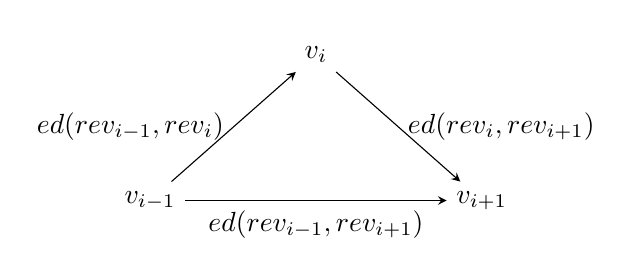
\begin{tikzpicture}
        \matrix (m) [matrix of math nodes, row sep=4em, column
          sep=4em]{ & v_i & \\ v_{i-1} & & v_{i+1}\\ };
        \path[-stealth] (m-2-1) edge node [left]
             {$ed(rev_{i-1},rev_i)$} (m-1-2) edge node [below]
             {$ed(rev_{i-1},rev_{i+1})$} (m-2-3) (m-1-2) edge node
             [right] {$ed(rev_i,rev_{i+1})$} (m-2-3); 
      \end{tikzpicture}\\ 
      \vspace{5mm}
      \textit{case a)} if $ed(rev_{i-1},rev_i) < ed(rev_{i-1},rev_i) +
      ed(rev_{i},rev_{i+1})$,\newline then $ed(rev_{i-1},rev_i)$ has been
      partially undone.\\
      \vspace{5mm}
      \textit{case b)} if $ed(rev_{i-1},rev_{i+1}) = 0$
      ($rev_{i-1} = rev_{i+1}$),\newline then $ed(rev_{i-1},rev_i)$ has been
      completely undone.\cite{Adler2007}
    \end{figure}
\end{frame}

  \section{The data}
  %%%%%%%%%%%%%%%%%%%%%%%%%%%%%%%%%%%%%%%%%%%%%%%%%%
  %%%%%%%%%%%%%%%%%%%%%%%%%%%%%%%%%%%%%%%%%%%%%%%%%%
  %%%%% 
  %%%%% GETTING / STORING THE DATA
  %%%%%
  %%%%%%%%%%%%%%%%%%%%%%%%%%%%%%%%%%%%%%%%%%%%%%%%%%
  %%%%%%%%%%%%%%%%%%%%%%%%%%%%%%%%%%%%%%%%%%%%%%%%%%
  \subsection{The Wikipedia API}
  \begin{frame}
    \frametitle{The Wikipedia API}
    
    \begin{quote}
      The MediaWiki web API is a Web service that provides convenient
      access to wiki features, data, and meta-data over HTTP.
    \end{quote}

    \onslide<1->{
    
      Ostensibly:
      \begin{itemize}
      \item Public access to all Wikipedia data
      \item Wide array of features 
      \end{itemize}
    
    }

    \onslide<2->{
    
      However:
      \begin{itemize}
      \item Mainly caters for bot-work
      \item Unreliable for our work
      \end{itemize}
      Accordingly, existing software not exactly what we're looking
      for.  

    }
 
  \end{frame}
  
  \subsection{Fetching procedure}
  \begin{frame}[fragile]{Alogrithm for fetching a \\revision history}    
        \tiny  
      \begin{algorithmic}
        \tiny
          \Procedure{Fetch}{$pageid$}
          \State $corrupt,visitedpages \gets \emptyset , \emptyset$
          \State $revid \gets 0$
          \State $parentid \gets wiki.getlatest(pageid)$
          \While{$revid \ne 0$ AND $revid \notin visitedpages$}\label{datal1} 
          \If{$revid$ is in the database}
          \State $parentid \gets database.getparentid(revid)$
          \Else
          \State $pagedata \gets wiki.getpage(revid)$
          \EndIf
          \If{$pagedata$ is corrupt}\label{datal3}
          \If{corruptness is recoverable}
          \State $corruptpages \gets + (revid, parentid, domain)$
          \Else
          \State terminate fetch\label{datal4}
          \EndIf
          \Else
          \State $database \gets page data$
          \EndIf
          \State $visitedpages \gets + (revid, domain)$
          \State $revid \gets parentid$\label{datal2}
          \EndWhile
          \ForAll {$(revision, parent, domain) \in corrupt$}
          \State $CorruptClean(revision, parent, domain)$
          \EndFor
          \State Mark $pageid$ as complete in $database$
          \EndProcedure
        \end{algorithmic}
\end{frame}

\note{Discoverable history. Is a little annoying, but fine as a data
  source}

\subsection{Database storage}
\begin{frame}[fragile]{Our database}
\begin{figure}[b]
  \tiny
  \centering
  \begin{subfigure}[t]{0.3\linewidth}
    \centering
    \begin{tabular}{ccc}
      \toprule
      \underline{revid} & \underline{domain} & content\\
      \midrule
      $\vdots$ & $\vdots$ & $\vdots$\\
    \end{tabular}
    \caption{\tiny Table: wikicontent}
  \end{subfigure}
  \hspace{2mm}
  \begin{subfigure}[t]{0.2\linewidth}
    \centering
    \begin{tabular}{cc}
      \toprule
      \underline{pageid} & \underline{domain} \\
      \midrule
      $\vdots$ & $\vdots$\\
    \end{tabular}
    \caption{\tiny Table:~wikifetched}
  \end{subfigure}
  \hspace{2mm}
  \begin{subfigure}[t]{0.4\linewidth}
    \centering
    \begin{tabular}{cccc}
      \toprule
      \underline{revid1} & \underline{revid2} & \underline{domain} & distance\\
      \midrule
      $\vdots$ & $\vdots$ & $\vdots$ & $\vdots$ \\
    \end{tabular}
    \caption{\tiny Table: wikitrajectory}
  \end{subfigure}\\
  \vspace{2mm}
  \begin{subfigure}[b!]{\linewidth}
    \centering
    \begin{tabular}{ccccccccc}
      \toprule
      \underline{revid} & \underline{domain} & pageid & title & username & userid & time & size &
      comment \\ 
      \midrule
      $\vdots$ & $\vdots$ & $\vdots$ & $\vdots$ & $\vdots$ & $\vdots$ & $\vdots$
      & $\vdots$ & $\vdots$ \\
    \end{tabular}
    \caption{\tiny Table: wikirevisions}
  \end{subfigure}\\
  \vspace{2mm}
  \begin{subfigure}[b!]{\linewidth}
    \centering
    \begin{tabular}{ccccccccc}
      \toprule
      \underline{revid} & \underline{domain} & maths & citations & filesimages & links &
      structure & normal & gradient\\
      \midrule
      $\vdots$ & $\vdots$ & $\vdots$ & $\vdots$ & $\vdots$ & $\vdots$ &
      $\vdots$ & $\vdots$ & $\vdots$ \\
    \end{tabular}
    \caption{\tiny Table: wikiweights} 
  \end{subfigure}
  \caption{Schemata for the database used to store wikipedia data}
\end{figure}  
\end{frame}
  
  \section{The analysis}
  %%%%%%%%%%%%%%%%%%%%%%%%%%%%%%%%%%%%%%%%%%%%%%%%%%
  %%%%%%%%%%%%%%%%%%%%%%%%%%%%%%%%%%%%%%%%%%%%%%%%%%
  %%%%% 
  %%%%% ANALYSING THE DATA
  %%%%%
  %%%%%%%%%%%%%%%%%%%%%%%%%%%%%%%%%%%%%%%%%%%%%%%%%%
  %%%%%%%%%%%%%%%%%%%%%%%%%%%%%%%%%%%%%%%%%%%%%%%%%%

  \subsection{Edit distance}
  \begin{frame}
    \frametitle{Wikipedia diffs} 

    We analyse using a Levenshtein edit-distance calculation
    algorithm, rather than using native Wikipedia diff-ing measures
    which include: 
    \begin{itemize}
      \item Diff-ing
      \item Size change
      \item `Page blanked' flags
      \item `Undo' flag (when people clicked `revert' button)
    \end{itemize}

    \onslide<2->{
      
      However, measures are insufficient, and have only partial
      support from the Wikipedia API
      
    }
    
  \end{frame}

  \begin{frame}
    \frametitle{Levenshtein edit distance}

    \begin{figure}
      \vspace{5mm}
      \centering
      for the function $\mbox{lev}_{a,b}(|a|,|b|)$:\\
      $$\mbox{lev}_{a,b}(i,j) = 
      \left\{
      \begin{array}{ll}
        \mbox{max}(i,j) & \mbox{if }min(i,j) = 0\\
        \mbox{min}\left\{
        \begin{array}{lll}
          lev_{a,b}(i-1,j)+1\\
          lev_{a,b}(i,j-1)+1\\
          lev_{a,b}(i-1,j-1)+1_{(a_i{\neq}b_j)}
        \end{array}
        \right.
        & else 
      \end{array}
      \right.$$
      when $a_i = b_j$, $1_{(a_i{\neq}b_j)} = 1$\\
      when  $a_i \neq b_j$, $1_{(a_i{\neq}b_j)} = 0$
      \caption{The definition of Levenshtein edit distance.}
      \label{fig:levdef}
    \end{figure}

  \end{frame}

  \subsection{Pair-distance calculation}

%\newcommand\tinyv{\@setfontsize\tinyv{4pt}}
\begin{frame}{Splitting the text by wikimarkup}
  \only<1>{
  	We may identify the following types of text from their tags:
  	\begin{itemize}
  	\item Internal links
  \item External links
  \item Images
  \item Files
  \item Musical scores
  \item Math-formatted text (similar to Latex math environment)
  \item Section headings (of differing levels)
  \item `Citation Needed' tags
  \item `As of' tags (used for identification of age-sensitive
    information)
  \item Block quotes
  \item Tables
  \end{itemize}
  }
  \only<2>{
  We then group them logically, as follows:
  \begin{description}
  \item[Equation]\hfill\\
    Math-formatted text
  \item[Source validation]\hfill\\
    Block quotes, Citations, `Citation Needed' tags, `As of' tags
  \item[Links]\hfill\\
    Internal Links, External Links
  \item[Structural]\hfill\\ 
    Section headings, Tables\\
    It was found in 2005 that this, if anything, was the clearest
    difference between Wikipedia and commercial
    encyclopedias,\cite{Giles2005} supporting previous
    conjecture.\cite{Denning2005} The regexes in this group provide a
    simple way of noticing changes that affect structure.
  \end{description}
  }
\end{frame}

    \begin{frame}[fragile]{Splitting text by wiki-markup tags}
\begin{figure}
  \tiny
  \centering
  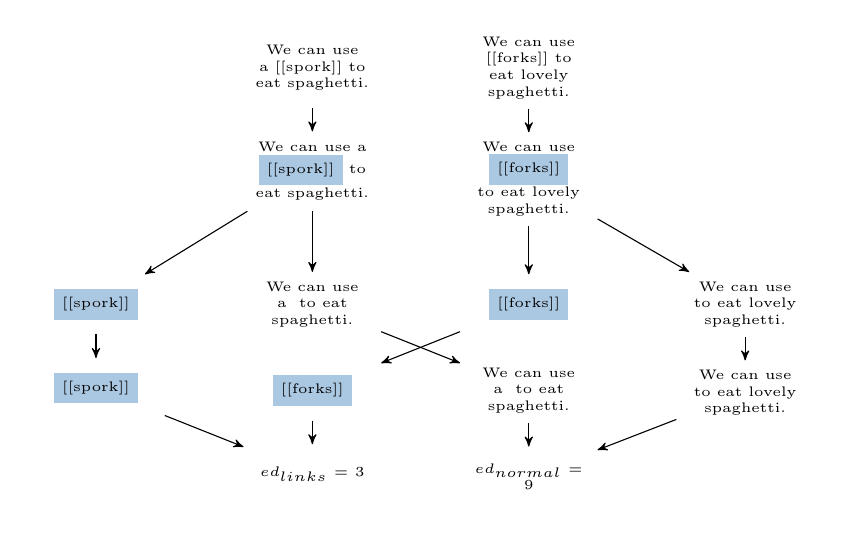
\begin{tikzpicture}[
      block1/.style={
        text width=1.5cm, 
        minimum height=1cm,
        align=center,
        anchor=north,
        font=\tiny,
      },
      block2/.style={
        text width=1.5cm, 
        minimum height=0.75cm,
        align=center,
        anchor=north,
        font=\tiny,
      }
    ]
    \node (a) [block1] {We can use a [[spork]] to eat spaghetti.};

    \node (b) [block1, right=1cm of a]{We can use [[forks]] to eat lovely
      spaghetti.};

    \node (c) [block1,below=0.3cm of a]{We can use a \hilight{[[spork]]} to eat
      spaghetti.};

    \node (d) [block1,below=0.3cm of b]{We can use \hilight{[[forks]]} to eat lovely
      spaghetti.};

    \node (e) [block2,below left=0.8cm and 1cm of c] {\hilight{[[spork]]}};
    
    \node (f) [block2,right=1cm of e] {We can use a\ \ to eat spaghetti.};

    \node (g) [block2,right=1cm of f] {\hilight{[[forks]]}};
    
    \node (h) [block2,right=1cm of g] {We can use\ \ to eat lovely spaghetti.};

    \node (i) [block2,below=0.3cm of e] {\hilight{[[spork]]}}; 
        
    \node (j) [block2,below=0.3cm of f] {\hilight{[[forks]]}}; 
    
    \node (k) [block2,below =0.3cm of g] {We can use a\ \ to eat
      spaghetti.};

    \node (l) [block2,below =0.3cm of h] {We can use\ \ to eat lovely spaghetti.};

    \node (m) [block2,below= 0.3cm of j] {$ed_{links} = 3$};

    \node (n) [block2,below =0.3cm of k] {$ed_{normal} = 9$};

    \draw [->] (a) -- (c);
    \draw [->] (b) -- (d);
    \draw [->] (c) -- (e);
    \draw [->] (c) -- (f);
    \draw [->] (d) -- (g);
    \draw [->] (d) -- (h);
    \draw [->] (e) -- (i);
    \draw [->] (g) -- (j);
    \draw [->] (f) -- (k);
    \draw [->] (h) -- (l);
    \draw [->] (i) -- (m);
    \draw [->] (j) -- (m);
    \draw [->] (k) -- (n);
    \draw [->] (l) -- (n);

  \end{tikzpicture}
  \caption{Diagram identification of link text, splitting text into
    normal and link segments, and performing separate levenshtein
    distance calculations}
\label{fig:split-diff}
\end{figure}
\end{frame}

\begin{frame}{Algorithm for processing split levenshtein distance}
  \tiny
  \begin{algorithmic}
    \State $regexes \gets $\{
    \Statex \tab`math1': `$<$math$>$((?!$<${\textbackslash}/math$>$).)*$<${\textbackslash}/math$>${\textbackslash}S',
    \Statex \tab`math2': `\{\{math((?!\}\}).)*\}\}',
    \Statex \tab`bquote': `$<$blockquote$>$((?!$<${\textbackslash}/blockquote$>$).)*$<${\textbackslash}/blockquote$>${\textbackslash}S',...
    \Statex\}\Comment{Regexes that recognise single Wikimarkup tags}
    \State $reggroups \gets $\{\label{dist-calc-groups}
    \Statex  \tab`maths':(regexes[`math1'], regexes[`math2']),...
    \Statex \}\Comment{Group of regexes by 'species'}
    \State $distances \gets \emptyset$
    \Function{PairDistance}{$str1,str2$}
    \State $strs \gets [str1, str2]$
    \ForAll {$key, reg \in reggroups$}
    \State $comparestr \gets [\emptyset , \emptyset]$
    \For {$i \gets 0,1$}
    \State $matches \gets reg.matches(strs[i])$
    \ForAll {$m \in matches$}
    \State $match, strs[i] \gets $extractsplit($m.start, m.end, strs[i]$)
    \State $comparestr[i] \gets comparestr[i] + match$
    \EndFor
    \EndFor
    \If {length($comparestr[0]$)$ > 0$ OR length($comparestr[1]$)$ > 0$}
    \State $distances[key] \gets LevDist(comparestr[0], comparestr[1])$ \Comment{See algorithm~\ref{lev-dist}}\label{mprocess-spawn}
    \Else
    \State $distances[key] \gets 0$
    \EndIf
    \EndFor
    \State $distances[$`$norm$'$] \gets LevDist(strs[0], strs[1])$
    \Comment{Process the remainder}
    \State return $distances$\label{mprocess-return}
    \EndFunction
  \end{algorithmic}
\end{frame}

  \subsection{Trajectory calculation}
  
  \begin{frame}
    \frametitle{Understanding context}
    
    We want to augment our first measure by analysing context. Our
    steps are:
    \begin{itemize}
      \item Take the final revision
      \item Compare to every revision in turn
    \end{itemize}
    
    \onslide<3->{
      The result is a map of how close each version was to the final
      at each point:
      
        \centering
        \pgfplotsset{width=0.5\textwidth}
        \begin{tikzpicture}
          \begin{axis}[
              title={\tiny Dummy revision history},
              ylabel={\tiny Ed. distance from final},
              xlabel={\tiny revision ID},
            ]
            \addplot [navyblue] table {dat/dummy_history.dat};
            \addplot [navyblue, only marks] table {dat/dummy_history.dat};
          \end{axis}
        \end{tikzpicture}
    }

  \end{frame}

  \begin{frame}
    
    \begin{columns}[c]
      \column{0.5\linewidth}
      \pgfplotsset{width=1\linewidth}
      \begin{tikzpicture}
        \begin{axis}
          \addplot [navyblue] table {dat/dummy1.dat};
          \addplot [redi] table {dat/dummy2.dat};
          \addplot [navyblue] table {dat/dummy3.dat};
          \addplot [navyblue, only marks] table {dat/dummy4.dat};
        \end{axis}
      \end{tikzpicture}

      \pgfplotsset{width=1\linewidth}
      \begin{tikzpicture}
        \begin{axis}
          \addplot [navyblue] table {dat/dummy1.dat};
          \addplot [redi] table {dat/dummy5.dat};
          \addplot [navyblue] table {dat/dummy6.dat};
          \addplot [navyblue, only marks] table {dat/dummy4.dat};
          \fill [greeni!25,fill opacity=0.5] (axis cs:4,13) rectangle (rel axis
          cs:1,0);
          \addplot[redi,dashed,update limits=false] 
          coordinates {(-2,13) (14,13)};
          \addplot[redi,dashed,update limits=false] 
          coordinates {(4,-2) (4,23)};
        \end{axis}
      \end{tikzpicture}
      
      \column{0.5\linewidth}
      \pgfplotsset{width=1\linewidth}
      \begin{tikzpicture}
        \begin{axis}
          \addplot [navyblue] table {dat/dummy1.dat};
          \addplot [redi] table {dat/dummy7.dat};
          \addplot [navyblue] table {dat/dummy6.dat};
          \addplot [navyblue, only marks] table {dat/dummy8.dat};
          \fill [greeni!25,fill opacity=0.5] (axis cs:4,13) rectangle (rel axis
          cs:1,0);
          \addplot[redi,dashed,update limits=false] 
          coordinates {(-2,13) (14,13)};
          \addplot[redi,dashed,update limits=false] 
          coordinates {(4,-2) (4,23)};
        \end{axis}
      \end{tikzpicture}

    \end{columns}
\end{frame}


  \begin{frame}
  
    \begin{figure}{Defining gradient factor}
      \tiny
      \centering
      \begin{subfigure}[b]{\linewidth}
        \tiny
        \centering
        \[gfactor(\Delta x,\Delta y) = \left\{ 
        \begin{array}{l l l}
          1 & \quad \text{if ${\Delta}x = 0$ and ${\Delta}y < 0$ }\\
          0 & \quad \text{if ${\Delta}x = 0$ and ${\Delta}y >= 0$ }\\
          \frac{arctan({\Delta}y/{\Delta}x)}{\pi}&\quad\text{if ${\Delta}x > 0$}
        \end{array} \right.\]
      \caption{\tiny gradient factor definition, with $\Delta x$ as
        change in time and $\Delta y$ as difference in to-final edit
        distance}
      \end{subfigure}\\
      \vspace{10mm}
      \onslide<2>{
        \begin{subfigure}[b]{\linewidth}
          \tiny
          \centering
          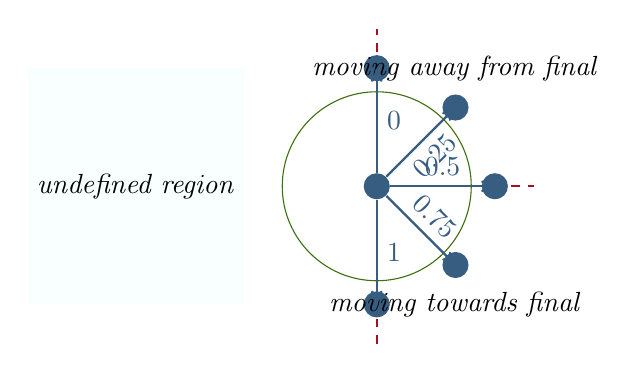
\begin{tikzpicture}[x=0.5cm,y=0.5cm]

            \draw[thick,redi,dashed] (4,0) -- (4,1);
            \draw[thick,redi,dashed] (4,7) -- (4,8);
            \draw[thick,redi,dashed] (7,4) -- (8,4);
            \draw [greeni] (4,4) circle (1.2cm);
            \node[fill,navyblue,circle] at (4,4) (o) {};
            \node[fill,navyblue,circle] at (7,4) (a) {};
            \node[fill,navyblue,circle] at (6,2) (b) {};
            \node[fill,navyblue,circle] at (6,6) (c) {};
            \node[fill,navyblue,circle] at (4,1) (d) {};
            \node[fill,navyblue,circle] at (4,7) (e) {};
            
            \node[fill=owhite,left=1.5cm of o, minimum height=3cm]{\textit{undefined region}};
            \node at (6,7) {\textit{moving away from final}};
            \node at (6,1) {\textit{moving towards final}};
            
            \draw [thick, navyblue, ->] (o) -- (7,4) node[sloped, midway, above]{$0.5$};
            \draw [thick, navyblue, ->] (o) -- (6,2) node[sloped, midway, above]{$0.75$};
            \draw [thick, navyblue, ->] (o) -- (6,6) node[sloped, midway, below]{$0.25$};
            \draw [thick, navyblue, ->] (o) -- (4,1) node[midway, right]{$1$};
            \draw [thick, navyblue, ->] (o) -- (4,7) node[midway, right]{$0$};
          \end{tikzpicture}
          \caption{\tiny mapping gradient factor to an arc}
        \end{subfigure}
      }
    \end{figure}
  \end{frame}

  \begin{frame}{Algorithm for trajectory calculation}
      \begin{algorithmic}
        \tiny
        \Procedure{TrajectoryCalculation}{$revids, domain$}
        \State $target \gets $database.gettext($revids[-1]$)\Comment{Last revision in list is most recent}
        \For {$i \gets length(revids), 0$}
        \If{trajectory distance not already in database}
        \State $str1 \gets $database.gettext($revids[i]$)
        \State $dist \gets $LevDist($str1, target$)\Comment{See algorithm~\ref{lev-dist}}
        \State $database.inserttrajectoryinsert(dist)$    
        \EndIf
        \EndFor
        \For{$i \gets 0, length(revids)$}
        \State $dist2 \gets $database.gettrajectory($revids[i],domain$)
        \State $dist1 \gets$
        \LineIf{database.gettrajectory($revid[i-1],domain$)}{$i \neq 0$}{$2 \times disty$}
        \State $time2 \gets $database.gettimestamp($revid[i],domain$)
        \State $time1 \gets $
        \LineIf{database.gettimestamp($revid[i-1],domain$)}{$i \neq 0$}{$timex$} 
        \State ${\Delta}x \gets time2 - time1$
        \State ${\Delta}y \gets dist2 - dist1$
        \If{${\Delta}x > 0$}
        \State $gradient = \frac{arctan({\Delta}y/{\Delta}x)}{\pi}$ 
        \ElsIf{$x = 0$}
        \State $gradient = $\LineIf{1}{$y < 0$}{0}
        \EndIf
        \State database.insertgradient($revid[i],domain,gradient$)
        \EndFor
        \EndProcedure
      \end{algorithmic}
  \end{frame}

  \section{Findings}
  %%%%%%%%%%%%%%%%%%%%%%%%%%%%%%%%%%%%%%%%%%%%%%%%%%
  %%%%%%%%%%%%%%%%%%%%%%%%%%%%%%%%%%%%%%%%%%%%%%%%%%
  %%%%% 
  %%%%% OUR FINDINGS
  %%%%%
  %%%%%%%%%%%%%%%%%%%%%%%%%%%%%%%%%%%%%%%%%%%%%%%%%%
  %%%%%%%%%%%%%%%%%%%%%%%%%%%%%%%%%%%%%%%%%%%%%%%%%%

  \section{References}
  \begin{frame}[allowframebreaks] %allow to expand references to multiple frames (slides)
    \frametitle{References}
    \scriptsize{\bibliographystyle{plain}}
    \bibliography{presentation} %bibtex file name without .bib extension
  \end{frame}

\end{document}
